\documentclass[]{IEEEtran}

% Your packages go here
\usepackage[utf8]{inputenc}
\usepackage{graphicx}
\usepackage{float}
\usepackage{listings}
\usepackage{xcolor}
\usepackage{mathrsfs}
\usepackage{amsmath}
%listings settings
\definecolor{codegreen}{rgb}{0,0.6,0}
\definecolor{codegray}{rgb}{0.5,0.5,0.5}
\definecolor{codepurple}{rgb}{0.58,0,0.82}
\definecolor{backcolour}{rgb}{0.95,0.95,0.92}
\definecolor{codeblue}{rgb}{0,0.8,0.99}
\definecolor{codeyellow}{rgb}{0.6,0.5,0}


\lstdefinestyle{vim_like}{
  backgroundcolor=\color{backcolour},   
  commentstyle=\color{codegreen},
  keywordstyle=\color{codeyellow},
  numberstyle=\tiny\color{codegray},
  stringstyle=\color{codepurple},
  basicstyle=\ttfamily\footnotesize,
  breakatwhitespace=false,         
  breaklines=true,                 
  captionpos=b,                    
  keepspaces=true,                 
  numbers=left,                    
  numbersep=5pt,                  
  showspaces=false,                
  showstringspaces=false,
  showtabs=false,                  
  tabsize=2
}
\lstset{style=vim_like}

\markboth{MO443 Digital Image Processing}{}

\begin{document}
  \title{Project 3 - Measures}
  \author{Thales Mateus Rodrigues Oliveira (RA 148051)
    \thanks{ra148051@students.ic.unicamp.br}
  }
  \maketitle
  
  \begin{abstract}
    In this project, it was given the task of calculating measures of objects within digital images. To fulfill the requirements, the solution implements four different algorithms, one for each required task from the project description\cite{PROJECT:3}. It was able to generate the outputs needed, and the implementation decisions are explained in this report.
  \end{abstract}
  
\section{Introduction}
The capability of identifying objects within digital images is a great step for automatic processing, segmentation, acquirement of statistic data, and so on. In order to obtain measures from objects within an image, some previous processing can be done to facilitate the calculations, such as identification of the contours of the objects. The goal of this work is to implement algorithms which return measures from objects within an image, and the auxiliar functions to do so. The next sections explains the implemented algorithm, the experiments realized and the output analysis
\par The code, along with the input files and the report is delivered in the compressed file THALES\_MATEUS\_RODRIGUES\_OLIVEIRA\_148051.tar, in the Google Classroom.

\section{The Program}
 
The program was implemented with Python 3.7.3. The libraries used and their respective versions are OpenCV 4.1.0, Numpy 1.16.4 and MatPlotLib 3.1.0.

\subsection{How to execute it}

The project has a Makefile available to help performing some actions on it. The Makefile has 3 basic instructions: clean, build and exec. Clean instruction removes generated images stored in the \textbf{output} folder, the execution code in \textbf{bin} folder and the folders itself. The Build instruction creates the \textbf{output} and \textbf{bin} folders, and moves the source code to \textbf{bin}. The Exec instruction executes the code with images in the \textbf{input} folder. Listing \ref{code:makefile} provides examples of how to execute the three instructions in a terminal.
\begin{lstlisting}[language=sh, caption={Makefile usage example}, label={code:makefile}]
  #clean environment, deletes output and bin folders and their content
  make clean
  
  #prepare the environment for code execution
  make build 

  #executes code
  make exec
\end{lstlisting}

\subsection{Input}

The program does not have an input argument by default, the input images are listed in code, and they are expected to be stored in the \textbf{input} folder. Listing \ref{code:input} shows how images are listed to be executed in code. The $images$ tuple is implemented in $src/main.py$.
\par The images are expected to be in the \textit{.png} format. The images in this work are expected to have objects in white background.

\begin{lstlisting}[language=Python, caption={Input images inside code}, label={code:input}]
  # for inserting other images, add tem to /input folder and list them here
  images = (
      'image-0',
      'image-1',
      'image-2'
  )
\end{lstlisting}

\subsection{Output}
The output of the program is a series of images describing the prior steps to measures acquirement, the measures themselves in the standard output, and a histogram containing measures' information, for each image input. The output images are saved in the \textbf{/output} folder. \textit{\textless image-name\textgreater-grayscale.png} stores the grayscale version of an input image, \textit{\textless image-name\textgreater-contours.png} stores only the contours of the objects in the input image, \textit{\textless image-name\textgreater-labeled.png} stores the labeled objects, and \textit{\textless image-name\textgreater-histogram.png} stores the histogram of areas of an input image.

\subsection{Implementation}
The functions which implement the prior and the measures operations are defined in the \textit{src/measures.py} file. The file has two auxiliary functions to calculate the measures: \textit{transform\_colors} and \textit{get\_contours}, which correspond to questions 1.1 and 1.2 in the project description. The \textit{get\_measures} function calculate the measures themselves, and relates to item 1.3 in the project description. The \textit{areas\_histogram} function builds the required histogram from item 1.4 from the description. The following items describe each of the implemented functions.

\subsubsection{Transform Colors}
The first prior task in order to obtain the measures was to transform the objects within the input image, which are colored, into their respective grayscale versions. In the output the objects are supposed to be painted in black, while the background remains the same. Listing \ref{code:transf-colors} shows the implementation. Vectorized operations were chosen to make the execution time faster.

\begin{lstlisting}[language=Python, caption={Transform Colors Implementation}, label={code:transf-colors}]
def transform_colors(img):
  b = g = r = img.copy()
  b[b[:, :, 0] < 255] = 0
  g[g[:, :, 1] < 255] = 0
  r[r[:, :, 2] < 255] = 0
  return b*g*r
\end{lstlisting}

\subsubsection{Contours of Objects}
The second task in order to obtain the measures was obtaining the contours of the objects within the image. The contours of the objects can be used to obtain measures such as area, perimeter and centroid of each object through the application of the chain rule to obtain the contours\cite{CLASS:1},\cite{CLASS:2}. Listing \ref{code:get-contours} shows the implementation of the method. The output is the image with only the contours of the objects drawn in red color, and the contour array itself. 

\begin{lstlisting}[language=Python, caption={Get Contours Implementation}, label={code:get-contours}]
def get_contours(img):
  contours_img = np.full_like(img, 255)

  _, thresh = cv2.threshold(img[:, :, 0], 127, 255, 0)
  contours, _ = cv2.findContours(thresh, cv2.RETR_TREE, cv2.CHAIN_APPROX_NONE)
  cv2.drawContours(contours_img, contours[1:], -1, (0, 0, 255), 1)
  return contours_img, contours
\end{lstlisting}

\subsubsection{Properties of Objects Extraction}
The measures calculation for the objects can be done entirely based on the contours obtained via Chain Rule. OpenCV has already built-in functions for area and perimeter calculation based on the contour (\textit{cv2.contourArea} and \textit{cv2.arcLength}, respectively). OpenCV also has a function for obtaining the moments of the objects (\textit{cv2.moments}). With the moments, the centroid coordinates can be obtained by applying the following relations:
\begin{equation}
  c_{x} = \dfrac{M_{10}}{M_{00}}
\end{equation}
 and 
\begin{equation}
  c_{y} = \dfrac{M_{01}}{M_{00}}
\end{equation},
where $(c_{x}, c_{y})$ are the centroid coordinates in x and y, respectively, $M_{00}$ is the order zero moment, and $M_{10}$ and $M_{01}$ are the first order moments.
\par After the measures calculation, the objects within the image are labeled, that label is placed in the image (the brightness of the image is changed to make the labels more readable), and the calculated properties are printed in the standard output. The return of the function is the labeled image and the calculated areas, which are used in the following step.
Listing \ref{code:meas} shows the main lines of the implementation.

\begin{lstlisting}[language=Python, caption={Properties Extraction Implementation}, label={code:meas}]
def get_measures(img, contours):
  ...
  # modify image colors to make the labels more readable
  hsv_img = cv2.cvtColor(img.copy(), cv2.COLOR_BGR2HSV)
  hsv_img[..., 2] = np.multiply(hsv_img[..., 2], 1.1).astype(np.uint8)
  output_img = cv2.cvtColor(hsv_img, cv2.COLOR_HSV2BGR) + 100

  idx = 0
  for contour in contours:
      # calculate required measures
      perimeter = cv2.arcLength(contour, True)
      area = cv2.contourArea(contour)
      moments = cv2.moments(contour)
      c_x = int(moments['m10']/moments['m00'])
      c_y = int(moments['m01']/moments['m00'])
      areas.append(area)

      # label image
      offset_x = 10 if idx > 9 else 5
      cv2.putText(output_img, str(idx), (c_x - offset_x, c_y + 5), font, 0.5, (0, 0, 0), 2)

      print("Region %2d: area: %6.1f perimeter: %9.5f " % (idx, area, perimeter))
      idx += 1
  return output_img, areas
\end{lstlisting}

\subsubsection{Histogram of Areas}
The last step was to generate a histogram of Areas of the objects, classifying the objects according to this specific constraint: Small regions are the ones with area less than $1500$, Medium regions are the ones with area between $1500$ and $3000$ and Big regions are the ones with area greater than $3000$. The number of objects with falls in each category is also displayed in the standard output. Matplotlib has a build-in function for histogram calculation (\textit{matplotlib.pyplot.hist}) that was used for both the plot and the standard output. Listing \ref{code:hist} shows the implementation.

\begin{lstlisting}[language=Python, caption={Histogram of Areas Implementation}, label={code:hist}]
def areas_histogram(areas, img_name):
  counts, _, _ = plt.hist(areas, [0, 1500, 3000, 4500], color='#0504aa',
                          alpha=0.7)
  plt.xlabel("Area")
  plt.ylabel("Numero de objetos")
  plt.title("Numero de objetos por area")
  plt.grid(axis='y', alpha=0.75)

  print("Classificacao dos objetos baseado em suas respectivas areas:")
  print("Numero de regioes pequenas: %d" % counts[0])
  print("Numero de regioes medias: %d" % counts[1])
  print("Numero de regioes grandes: %d" % counts[2])

  plt.savefig('output/' + img_name + "-histogram" + '.png')
  plt.show()
\end{lstlisting}

\section{Experiments}
The \textit{src/main.py} file executes the test pipeline. The idea is the following: for each input image, execute the four implemented functions mentioned in the previous section, and save their respective outputs. The input images are stored in \textbf{input} folder as mentioned before, and their names and dimensions are listed in table \ref{table:input}. The input images are shown in figure \ref{fig:input-images}. The generated output images are saved in $png$ extension.

\begin{table}[h!]
\centering
\begin{center}
\begin{tabular}{ |c|c| } 
 \hline
 Image Names & Dimensions (width x height) \\
 \hline
  image-0.png &  563 x 327\\ 
 \hline
  image-1.png & 563 x 343\\
 \hline
  image-2.png &  238 x 238\\ 
 \hline
\end{tabular}
\caption{Input images used in experiments}
\label{table:input}
\end{center}
\end{table}

\begin{figure}[]
  \centering
  \fbox{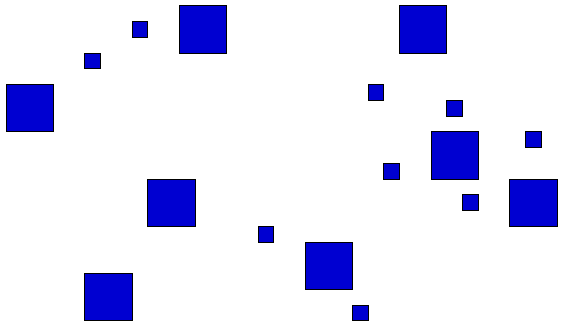
\includegraphics[width=0.3\hsize]{../input/image-0.png}}
  \fbox{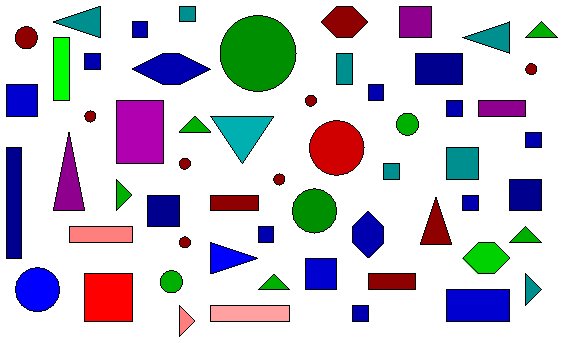
\includegraphics[width=0.3\hsize]{../input/image-1.png}}
  \fbox{
\includegraphics[width=0.2\hsize]{../input/image-2.png}}
  \caption{Input images used in experiments. a) image-0 b) image-1 c) image-2}
  \label{fig:input-images}
\end{figure}

As we have 3 input images, 4 implemented functions, we have 12 images of output, and 6 output text blocks. The output images are stored in the \textbf{output} folder.

\section{Discussion}
This section is organized in four parts, and they analyze the results of each function for all the input images.

\subsection{Transform colors}
The results of the method for all input images are shown in figure \ref{fig:transf-colors}. As it can be seen, the results are satisfatory, and they can be used for the contour calculation of each object.

\begin{figure}[]
  \centering
  \fbox{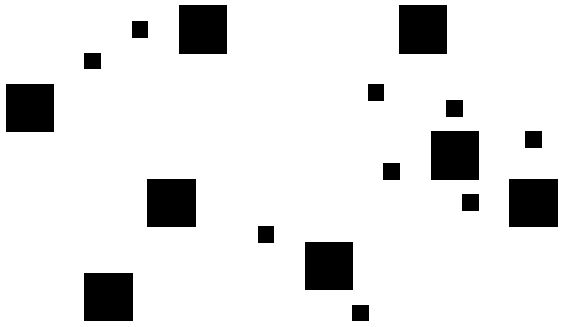
\includegraphics[width=0.3\hsize]{../output/image-0-grayscale.png}}
  \fbox{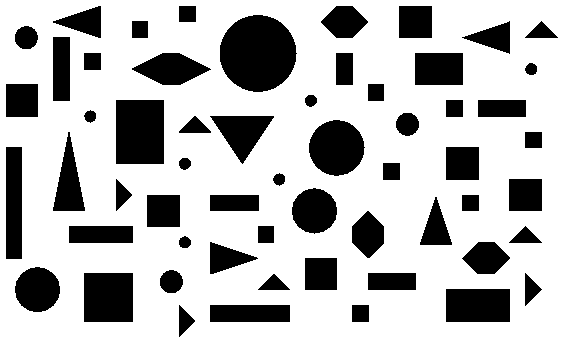
\includegraphics[width=0.3\hsize]{../output/image-1-grayscale.png}}
  \fbox{
\includegraphics[width=0.2\hsize]{../output/image-2-grayscale.png}}
  \caption{Transform Colors Results. a) image-0 b) image-1 c) image-2}
  \label{fig:transf-colors}
\end{figure}

\subsection{Contours of Objects}
The results of the method for all grayscale images obtained in the previous subsection are shown in figure \ref{fig:contours}. The painted contours seem to fit the objects in their respective original images, which validates the implementation. The obtained contours can be used in the following function.

\begin{figure}[]
  \centering
  \fbox{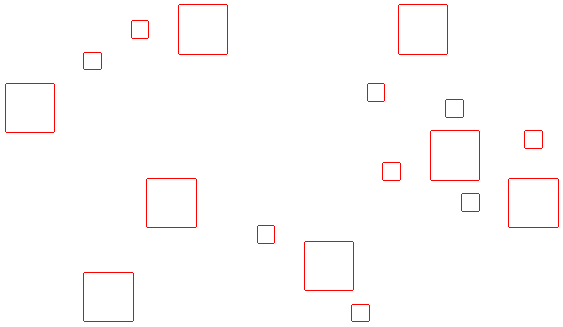
\includegraphics[width=0.5\hsize]{../output/image-0-contours.png}}
  \fbox{
\includegraphics[width=0.6\hsize]{../output/image-1-contours.png}}
  \fbox{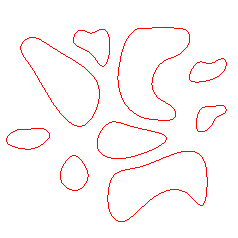
\includegraphics[width=0.4\hsize]{../output/image-2-contours.png}}
  \caption{Contours of Objects Results. a) image-0 b) image-1 c) image-2}
  \label{fig:contours}
\end{figure}

\subsection{Properties of Objects Extraction}
The figure results of the method for all images and their contours are show in figure \ref{fig:labeled}. As mentioned before, some brightness effect was applied in order to make the label readable. The label is placed in a way to center it related to the centroid position. The text outputs are shown in listing \ref{code:out-1-1}, \ref{code:out-1-2} and \ref{code:out-1-3} for images 0, 1 and 2 respectively. As it can be seen, small objects have small area and so on. 

\begin{figure}[]
  \centering
  \fbox{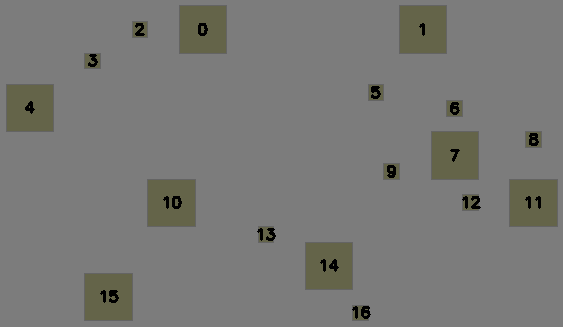
\includegraphics[width=0.8\hsize]{../output/image-0-labeled.png}}
  \fbox{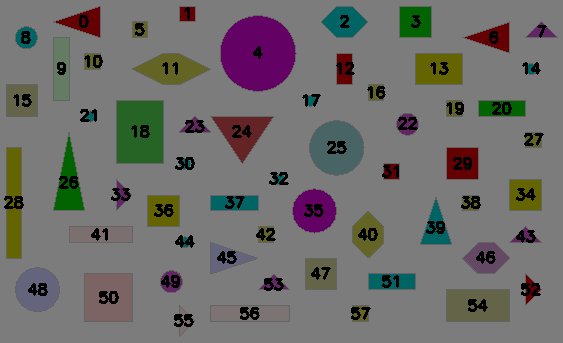
\includegraphics[width=0.8\hsize]{../output/image-1-labeled.png}}
  \fbox{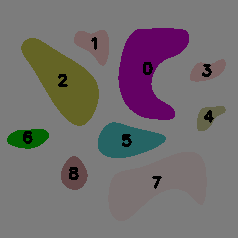
\includegraphics[width=0.4\hsize]{../output/image-2-labeled.png}}
  \caption{Properties of Objects Figure Results. a) image-0 b) image-1 c) image-2}
  \label{fig:labeled}
\end{figure}

\begin{lstlisting}[language=sh, caption={Output for Extracted Properties for Image 0}, label={code:out-1-1}]
  Region  0: area: 2448.0 perimeter: 195.65685 
  Region  1: area: 2448.0 perimeter: 195.65685 
  Region  2: area:  304.0 perimeter:  67.65685 
  Region  3: area:  304.0 perimeter:  67.65685 
  Region  4: area: 2399.0 perimeter: 193.65685 
  Region  5: area:  304.0 perimeter:  67.65685 
  Region  6: area:  322.0 perimeter:  69.65685 
  Region  7: area: 2448.0 perimeter: 195.65685 
  Region  8: area:  322.0 perimeter:  69.65685 
  Region  9: area:  322.0 perimeter:  69.65685 
  Region 10: area: 2448.0 perimeter: 195.65685 
  Region 11: area: 2448.0 perimeter: 195.65685 
  Region 12: area:  322.0 perimeter:  69.65685 
  Region 13: area:  304.0 perimeter:  67.65685 
  Region 14: area: 2399.0 perimeter: 193.65685 
  Region 15: area: 2448.0 perimeter: 195.65685 
  Region 16: area:  304.0 perimeter:  67.65685   
\end{lstlisting}

\begin{lstlisting}[language=sh, caption={Output for Extracted Properties for Image 1}, label={code:out-1-2}]
  Region  0: area:  880.0 perimeter: 144.08326 
  Region  1: area:  304.0 perimeter:  67.65685 
  Region  2: area: 1072.0 perimeter: 124.50967 
  Region  3: area: 1120.0 perimeter: 131.65685 
  Region  4: area: 4724.0 perimeter: 256.93607 
  Region  5: area:  304.0 perimeter:  67.65685 
  Region  6: area:  849.0 perimeter: 144.91169 
  Region  7: area:  322.0 perimeter:  82.91169 
  Region  8: area:  452.0 perimeter:  79.59798 
  Region  9: area: 1168.0 perimeter: 163.65685 
  Region 10: area:  322.0 perimeter:  69.65685 
  Region 11: area: 1631.5 perimeter: 187.92388 
  Region 12: area:  592.0 perimeter:  99.65685 
  Region 13: area: 1615.0 perimeter: 161.65685 
  Region 14: area:  130.0 perimeter:  42.62742 
  Region 15: area: 1120.0 perimeter: 131.65685 
  Region 16: area:  304.0 perimeter:  67.65685 
  Region 17: area:  129.5 perimeter:  42.04163 
  Region 18: area: 3183.0 perimeter: 225.65685 
  Region 19: area:  322.0 perimeter:  69.65685 
  Region 20: area:  880.0 perimeter: 131.65685 
  Region 21: area:  128.0 perimeter:  43.45584 
  Region 22: area:  450.0 perimeter:  79.59798 
  Region 23: area:  337.0 perimeter:  82.08326 
  Region 24: area: 1647.5 perimeter: 188.75231 
  Region 25: area: 2480.0 perimeter: 186.99495 
  Region 26: area: 1423.0 perimeter: 206.08326 
  Region 27: area:  304.0 perimeter:  67.65685 
  Region 28: area: 1919.0 perimeter: 257.65685 
  Region 29: area: 1154.0 perimeter: 133.65685 
  Region 30: area:  129.5 perimeter:  42.04163 
  Region 31: area:  322.0 perimeter:  69.65685 
  Region 32: area:  129.0 perimeter:  43.45584 
  Region 33: area:  304.0 perimeter:  80.08326 
  Region 34: area: 1120.0 perimeter: 131.65685 
  Region 35: area: 1647.0 perimeter: 153.19596 
  Region 36: area: 1120.0 perimeter: 131.65685 
  Region 37: area:  848.0 perimeter: 131.65685 
  Region 38: area:  304.0 perimeter:  67.65685 
  Region 39: area:  880.0 perimeter: 144.08326 
  Region 40: area: 1087.5 perimeter: 125.09545 
  Region 41: area: 1168.0 perimeter: 163.65685 
  Region 42: area:  304.0 perimeter:  67.65685 
  Region 43: area:  322.0 perimeter:  82.91169 
  Region 44: area:  129.0 perimeter:  42.62742 
  Region 45: area:  878.5 perimeter: 143.49747 
  Region 46: area: 1088.5 perimeter: 125.92388 
  Region 47: area: 1087.0 perimeter: 129.65685 
  Region 48: area: 1640.0 perimeter: 152.36753 
  Region 49: area:  452.0 perimeter:  79.59798 
  Region 50: area: 2498.0 perimeter: 197.65685 
  Region 51: area:  880.0 perimeter: 131.65685 
  Region 52: area:  322.0 perimeter:  82.91169 
  Region 53: area:  304.0 perimeter:  80.08326 
  Region 54: area: 2208.0 perimeter: 195.65685 
  Region 55: area:  304.0 perimeter:  80.08326 
  Region 56: area: 1456.0 perimeter: 195.65685 
  Region 57: area:  322.0 perimeter:  69.65685   
\end{lstlisting}

\begin{lstlisting}[language=sh, caption={Output for Extracted Properties for Image 2}, label={code:out-1-3}]
  Region  0: area: 4107.0 perimeter: 319.42135 
  Region  1: area:  843.5 perimeter: 125.63961 
  Region  2: area: 3690.5 perimeter: 265.11984 
  Region  3: area:  584.0 perimeter: 104.91169 
  Region  4: area:  478.0 perimeter:  94.42641 
  Region  5: area: 1761.5 perimeter: 179.78174 
  Region  6: area:  688.5 perimeter: 108.66905 
  Region  7: area: 4067.0 perimeter: 311.07821 
  Region  8: area:  716.5 perimeter: 101.98276 
\end{lstlisting}

\subsection{Histogram of Areas}
Figure \ref{fig:hist} shows the histograms for all input images, and listing \ref{code:out-2-1}, \ref{code:out-2-2} and \ref{code:out-2-3} the respective outputs as desired. It is possible to analyze that, based on the areas obtained in the previous function, the histogram calculation is able to separate each object in its respective category. 

\begin{figure}[]
  \centering
  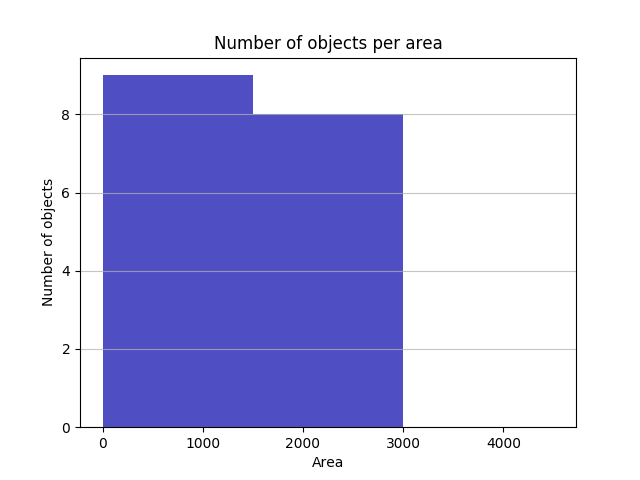
\includegraphics[width=0.8\hsize]{../output/image-0-histogram.png}
  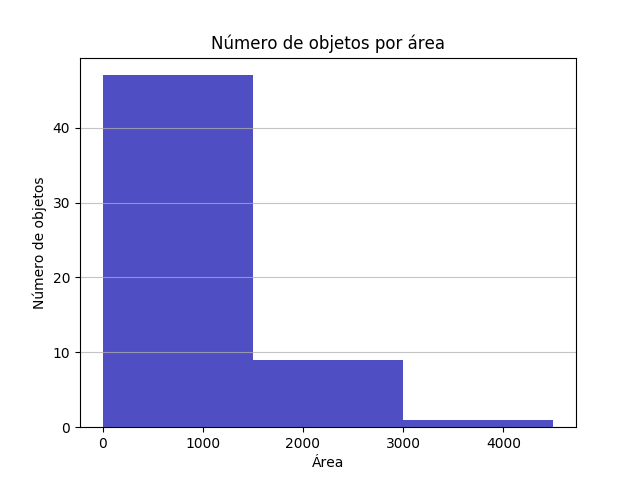
\includegraphics[width=0.8\hsize]{../output/image-1-histogram.png}
  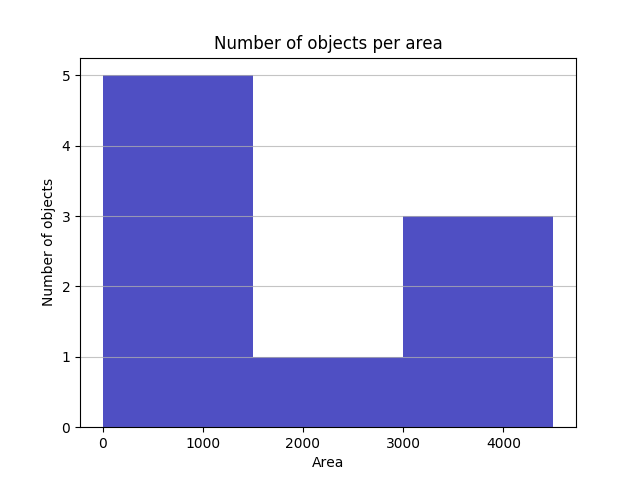
\includegraphics[width=0.8\hsize]{../output/image-2-histogram.png}
  \caption{Histogram of object areas. a) image-0 b) image-1 c) image-2}
  \label{fig:hist}
\end{figure}

\begin{lstlisting}[language=sh, caption={Output for Histogram of Areas for Image 0}, label={code:out-2-1}]
  Classification of objects based on their respective areas:
  Number of small regions: 9
  Number of medium regions: 8
  Number of big regions: 0
\end{lstlisting}

\begin{lstlisting}[language=sh, caption={Output for Histogram of Areas for Image 1}, label={code:out-2-2}]
  Classification of objects based on their respective areas:
  Number of small regions: 47
  Number of medium regions: 9
  Number of big regions: 1  
\end{lstlisting}

\begin{lstlisting}[language=sh, caption={Output for Histogram of Areas for Image 2}, label={code:out-2-3}]
  Classification of objects based on their respective areas:
  Number of small regions: 5
  Number of medium regions: 1
  Number of big regions: 3  
\end{lstlisting}

\section{Conclusion}
The properties extraction from objects within images was possible thanks to the approaches presented in the academia.
The usage of different input images made it possible to validate the implementation for different object shapes. Future work could be done to generalize the methodology for different background and object colors/textures. 

\bibliography{ref-project}
\bibliographystyle{ieeetr}

\end{document}
